\section{Ablation Study}
\label{sec:ablation}

\subsection{Direct Local Cues Are a Negative Control}

The first ablation asks whether the local reliability map can be used as an
anomaly map directly. It cannot. Direct wavelet fusion is worse than the final
method on MVTec and VisA, and is also worse than semantic-only prototype
adaptation. This supports the method boundary in Sec.~\ref{sec:method}: local
high-frequency or boundary-aware responses are candidate cues, not final
evidence.

The GlobalRef diagnostic control is less pathological: it improves over direct
map fusion and over the fixed-prototype baseline on pixel AUPRO. However, it
still remains below the image-conditioned reference, with \method{} improving
pixel AUPRO over GlobalRef by $+1.9$ on MVTec and $+2.5$ on VisA. This is the
desired diagnostic pattern: a fixed global reference is useful, but it does not
replace a reference estimated from the current image.

\begin{figure}[t]
  \centering
  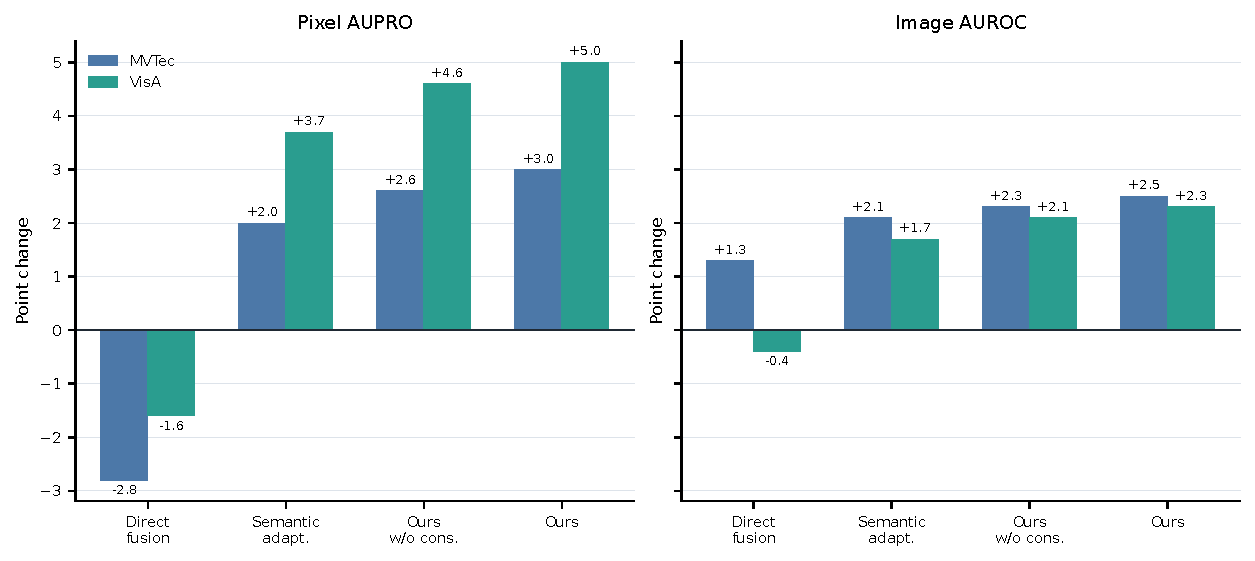
\includegraphics[width=\linewidth]{figures_ablation/figures/controlled_core_ablation_gain_bars.pdf}
  \caption{Controlled core ablation gains over the fixed baseline. Direct
  fusion is the negative control, GlobalRef tests a fixed reference, and
  semantic-only prototype adaptation is the strongest non-frequency
  image-conditioned control.}
  \label{fig:controlled-core-gains}
\end{figure}

\subsection{Reliability Design}

Table~\ref{tab:wavelet-design-ablation} isolates how the local reliability
signal is used. Semantic-only prototype adaptation uses $s_i^0$ without
$W_i$. HF-only reliability uses high-frequency magnitude without the
low-frequency boundary suppression. Boundary-aware reliability uses
Eq.~\eqref{eq:reliability}. The final method further adds conservative
prototype calibration.

\begin{table*}[t]
\centering
\caption{Wavelet reliability design ablation on MVTec and VisA. All metrics are reported in percent; the best result within each dataset and metric is marked in bold.}
\label{tab:wavelet-design-ablation}
\resizebox{\textwidth}{!}{%
\begin{tabular}{llcccc}
\toprule
Dataset & Variant & Pixel AUROC & Pixel AUPRO & Image AUROC & Image AP \\
\midrule
MVTec & Direct wavelet fusion & 88.7 & 80.4 & 92.9 & 96.9 \\
MVTec & Semantic-only prototype adaptation & 91.6 & 85.2 & 93.7 & 97.1 \\
MVTec & HF-only reliability + prototype adaptation & 91.6 & 85.3 & 94.0 & 97.2 \\
MVTec & Boundary-aware reliability + prototype adaptation & 91.7 & 85.7 & 93.8 & 97.3 \\
MVTec & Ours (unnamed) & \textbf{91.8} & \textbf{86.2} & \textbf{94.1} & \textbf{97.4} \\
\midrule
VisA & Direct wavelet fusion & 94.6 & 85.1 & 81.6 & 84.8 \\
VisA & Semantic-only prototype adaptation & 96.0 & 90.4 & 83.7 & 86.9 \\
VisA & HF-only reliability + prototype adaptation & 96.0 & 90.8 & 84.0 & 86.9 \\
VisA & Boundary-aware reliability + prototype adaptation & 96.1 & 91.2 & 83.9 & 87.1 \\
VisA & Ours (unnamed) & \textbf{96.2} & \textbf{91.7} & \textbf{84.3} & \textbf{87.3} \\
\bottomrule
\end{tabular}%
}
\end{table*}


\begin{figure}[t]
  \centering
  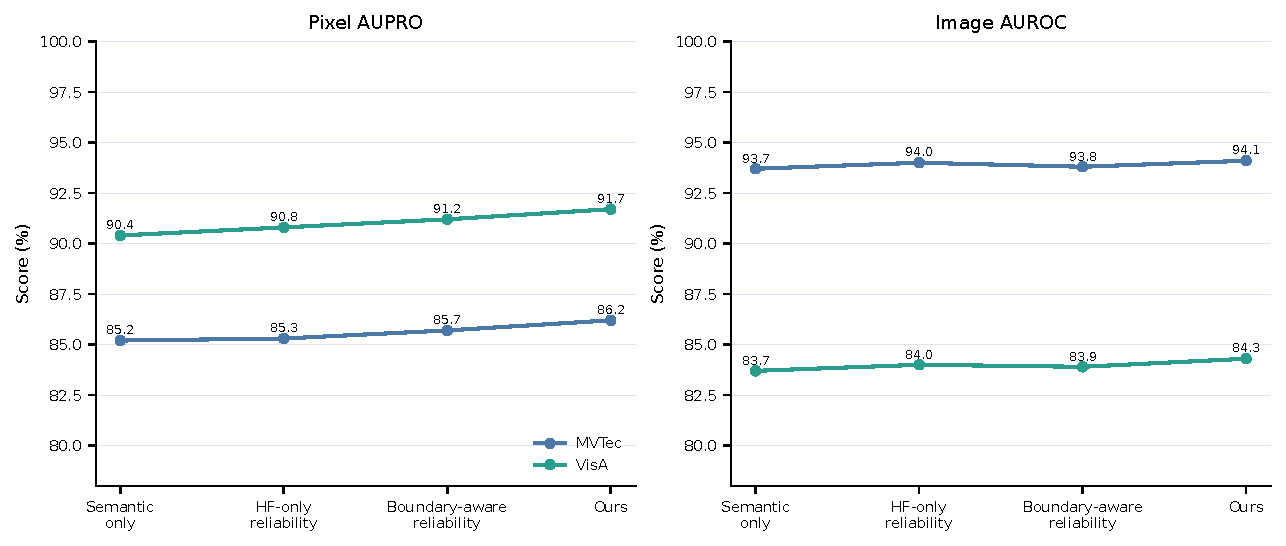
\includegraphics[width=\linewidth]{figures_ablation/figures/wavelet_design_ablation_progression_lines.pdf}
  \caption{Reliability-design ablation. The figure is used to check the
  evidence-selection mechanism, not to claim that a wavelet map is itself an
  anomaly detector.}
  \label{fig:wavelet-design-progression}
\end{figure}

\subsection{Conservative Calibration}

Prototype calibration can be harmful if unreliable abnormal patches are written
into the abnormal prototype. The current stable configuration therefore uses a
small normal-side update and disables effective abnormal-side updates
($\alpha_0=0$). Normal-image stability provides an additional sanity check:
the final method does not increase normal-image false-positive area over the
baseline.

\begin{table}[t]
  \centering
  \caption{Normal-image stability. FP area is the area above the corresponding
  threshold on normal images; lower is better.}
  \label{tab:normal-stability}
  \resizebox{\linewidth}{!}{%
  \begin{tabular}{llccc}
    \toprule
    Dataset & Method & Normal images & FP area @ p95 & FP area @ p99 \\
    \midrule
    MVTec & Baseline & 467 & 5.002\% & 1.001\% \\
    MVTec & \method{} & 467 & 4.895\% & 0.960\% \\
    VisA & Baseline & 962 & 4.996\% & 1.001\% \\
    VisA & \method{} & 962 & 4.718\% & 0.937\% \\
    \bottomrule
  \end{tabular}%
  }
\end{table}
